In this section we gonna analyze the meta data of the results of the systematic search. This will help us to identify research gaps and other trends that are going on in the field. First we gonna analyze the publication years and topics of the articles in the review.

In the final resulting literature subset we identified 86 relevant articles from which 84 articles where published in a Peer Reviewed Journal and 2 where published in conference proceedings. When looking at \ref{fig: publications_per_year_per_categories} we can see an increasing trend of publication from 2009 until 2021 with some ups and downs. This show the increasing importance of smartphone participants in web surveys in the last 10 years [citation]. As more and more people are having access to smartphones and are getting used to using them [citation], this trend was foreseeable. This is something one has to take into account when reading the results of the review that these are an snapshot of the past and the situation is dynamically evolving. On future research project is to update the results by repeating the experiments.

\begin{figure}
    \centering
    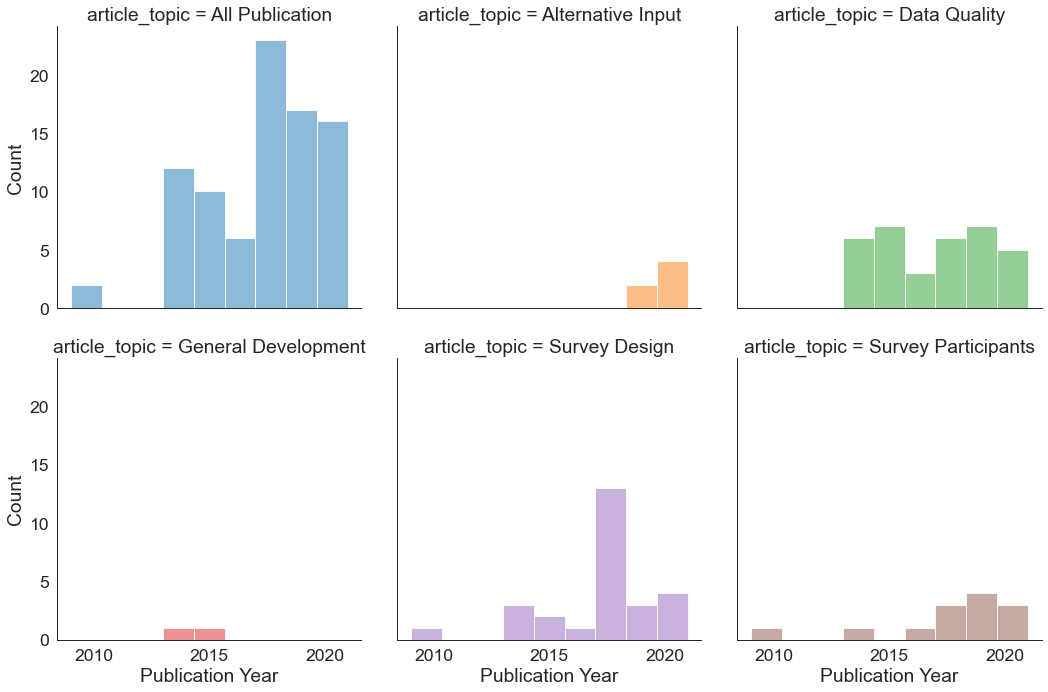
\includegraphics[width=\textwidth]{reports/figures/publications_per_year_per_categories.png}
     \caption{Graphic of the number of published articles per year per category of approach in the selected literature from 2008 to 2021}
    \label{fig: publications_per_year_per_categories}
\end{figure}

An interesting observation, that is important for our evaluation of the dimension of mobile web surveys, is the time difference between publication and data collection. As 74 articles in the review collected survey data, the time of survey taking is important for the evaluation of the results. As increasing smartphone penetration and improved usage changes the behaviour of smartphone user [citation]. When analyzing the year of survey execution we could identify an average gap between publication year and survey execution year of three years. This implies an important time lag of the data and the insight we gain in this review. As the latest survey was done in 2019 and 90\% of the survey were done in or before 2017. As we can see there is a lag in scientific publication and survey execution. That is significant if observe the fast consumer trends and the tremendously increasing trend of mobile usage and the changing landscape of tehcnology (smart watch, samrt phoene tc).

As only two publication were in conference proceedings and a large majority was published in peer reviewed journals we will limit us to an analysis of the published Journals. As one can observe in table \ref{tab: journals}, we have a classic power law distribution with the majority of publication concentraing on a few journals and the rest of publications scattered in various journals. There are no suprising journals in the list and an independent search of influential peer reviewed journals revealed no misisng journals.We missed howber an editorail reviewed journal with an medium impact on the journal in our review. This is  survey practice from the American Association for Public Opinion Research. If one does an review on a specific topic, one could decide to include grey literature and other scientific literatuer types.  Since an important point to mention is that there is a lot of grey scientigic literatuere that was not used in this article. For example the the AAPOR and Jorichasfa Conference. That influenced a lot of papers. They could be a vry interesting source, if one does a systematic review on a speciifc topic and wants to include a larger data base. They are however not necessary from th quality of a peer reviewed pubklication, that lead to thheir exclusion in this review.

\begin{table}
	\centering
	\begin{tabular}{ll}
		\toprule
		Author Name & Number of Articles \\
		\midrule
        Social Science Computer Review & 27\\
        International Journal of Market Research & 8\\
        Survey Research Methods& 6\\
        methods, data, analyses & 5\\
        Public Opinion Quarterly & 4\\
        International Journal of Social Research Methodology & 4\\
        Journal of Survey Statistics and Methodology & 4\\
        Field methods & 3\\
        Sociological Methods \& Research & 2\\
        Internet Research & 2 \\
        Quality \& Quantity  & 2\\
		\bottomrule 
	\end{tabular}
	\caption{Overview of the Journals with more than 2 publications in the review}
	\label{tab: journals}
\end{table}

When analysing the authors of the articles we see a similar pattern with a few very present authors and other authors that only contribute in one or two articles. The most publications are done by Mick P. Couper and Melanie Revilla. As the often publishing authors are also cooperting frequenlty one could make an netwo analysis to better understand the dynamic of the collobereations.We see the most influential authors make a lot of the papers. This correlates with countries and survey operators andlead to may a bias in the scientific literature. THe strong influence of the top authors on the literature in this review may induce an bias as we will discuss when analyzing the survey operators.

\begin{table}
	\centering
	\begin{tabular}{ll}
		\toprule
		Author Name & Number of Articles \\
		\midrule
		Couper, Mick P. &        15 \\
        Revilla, Melanie &      14\\
        Toepoel, Vera  &         8\\
        Lugtig, Peter   &        7\\
        Mavletova, Aigul    &    6\\
        Antoun, Christopher  &   6\\
        Bosch, Oriol J.   &      5\\
        De Bruijne, Marika  &    3\\
        Ochoa, Carlos      &     3\\
        Keusch, Florian     &    3\\
        Wang, Lin           &    3\\
        Buskirk, Trent D.     &  3\\
        Schlosser, Stephan  &   3\\
        Toninelli, Daniele   &   3\\
        Höhne, Jan K.        &   3\\
        Wijnant, Arnaud      &   3\\
        Roßmann, Joss       &    3\\
        Yan, Ting            &   3\\
		\bottomrule 
	\end{tabular}
	\caption{Overview of the authors with more than 3 publications in the review}
	\label{tab: authors}
\end{table}

As we have often the same survey operator and most of the surveys are executed by panelists, that are already profis in survey taking there may be a bias. They also have other incidents for taking the survey that also influences they work [citation]. This is on the one hand caused by the experience in survey taking, (what is allowed how to satiscify withoput punishment and how toexecute survey fast) [citation] One examßple is that in the centERpanel most of the time they take the survey on pc and already had a large learning curve for this format. Now they have to handle the mobile and have to swithc. Another big point is the incentive to complete a survey that may also alter the motivaiton and reudce breakoff rate and satisfcing beahvior. this is an effect that should be controlled in future studies. 

\begin{table}
	\centering
	\begin{tabular}{ll}
		\toprule
		Survey Operator Name & Number of Surveys \\
		\midrule
        Netquest & 12\\
        CentERdata &8\\
        Online Market Intelligence &5\\
        KnowledgePanel  &3\\
        GESIS &3\\
        German Longitudinal Election Study &3\\
        SurveyMonkey Audience  &2\\
        Amazon Mechanical Turk & 2\\
		\bottomrule 
	\end{tabular}
	\caption{Overview of the Professional Survey Operators used for more than one survey in the review}
	\label{tab: author}
\end{table}


Another important point in this review is the surveyed population in the executed surveys. As we already mentioned in the analysis of the authors that this correlates with the atuhros. We mapped the countries in \ref{fig: surveys_per_country}. We exclude survey with more than three countries as we cannot say anything about the representativity of the population by the survey and the real part. Theory: not all countries present that lead to bias, especially considering the tehcnical and societal standards in the socieities that were interviewed. As the developed countries have opther access to pc, mobile and tablet. In some developing countries there may be only access to a mobile phone inc onctrast to developed counmtries where still the access to pcis maybe more.  We can see an strong bias as most surveys (83\%) are taken in USA, Germany, Netherlands, Spain and Russia. Which lead to an coverage bias for other world regions as south america, africa, asia and australia. Also within europe there is an overreprsentativity of western countries missing south eastern countries. When analysising the results of the review one has to take into account the missing representativity of the results for these regions. This is also an possible future reserach endevaour to transfer the results to other world regions.

\begin{figure}
    \centering
    
\includegraphics[width=\textwidth]{reports/figures/surveys_per_country.png}
     \caption{Graphic of the number of survey per country}
    \label{fig: surveys_per_country}
\end{figure}


As we could see in this section in the analysis of the meta data of the articles in the review, there are few issues that one has to mind when interpreting the results in the upcoming section. We saw an increasing trend in research, that will most likely not stop in the next years, as the important of mobile internet is still increasing [citation]. We also saw that there is a lag in the time from survey operation to publicaiton of average three years, that we have to mind when interpreting the results. Other possible biases are induced by the concentration of authors and professional survey operators, that could possibly skew the results. One last important factor we have identified is the misisng representativity of the countries survey were operated in, so that the results of review are limited to a few countries. Therefore we have identified future reserach projects, where one reopreats the experiments in other countries and in newer time to test and eventually update the results. 






